\newpage
\section{PLANIFICACIÓN TEMPORAL Y PRESUPUESTO} \label{planificacion_presupuesto}

\subsection{Estructura de Descomposición del Proyecto}

La descomposición de este trabajo fin de grado puede realizarse dividiendo el mismo en 5 bloques fundamentales (en color naranja). Estos, a su vez, se subdividen en varios paquetes de trabajo (en color verde y azul). Cada paquete de trabajo tiene un alcance y contenido único, y se ejecuta en un período de tiempo y con un presupuesto determinados.

\begin{figure}[h]
    \centering
    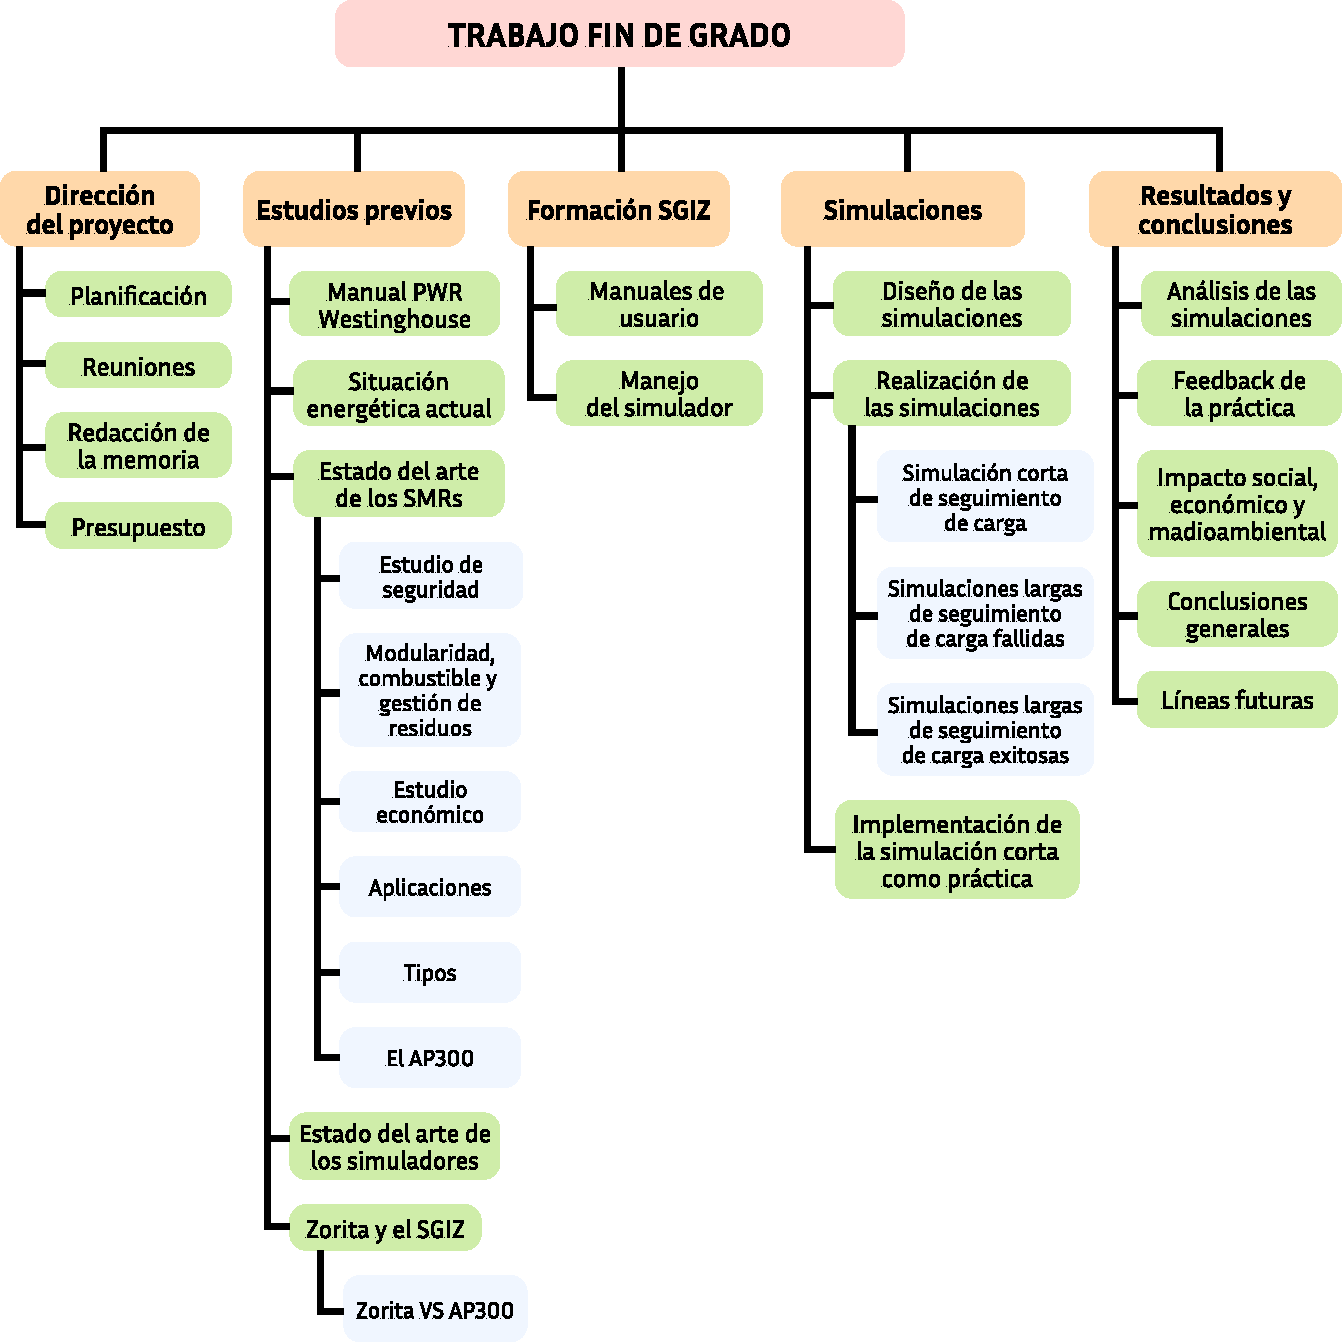
\includegraphics[width=\textwidth]{content/figures/edp_tfg.pdf}
    \caption{Estructura de Descomposición del Proyecto (EDP).}
    \label{fig:edp_tfg}
  \end{figure}

  Esta EDP proporciona la referencia básica para la elaboración del diagrama de Gantt, en el cual se incluye de forma detallada la evolución temporal del proyecto y de sus correspondientes paquetes de trabajo.

  \subsection{Diagrama de Gantt}

  A continuación, se detalla la tabla de la programación temporal del proyecto, a partir de la cual se realiza el diagrama de Gantt:

  \begin{table}[!h]
    \centering
    \begin{tabular}{|r|c|c|c|}
    \hline
    \rowcolor[HTML]{CBCEFB} 
    \textbf{Actividad}                                           & \textbf{Días}             & \textbf{Inicio}                   & \textbf{Final}                    \\ \hline
    \rowcolor[HTML]{FFCCC9} 
    \textbf{TRABAJO FIN DE GRADO}                                & \textbf{218}              & \textbf{1-2-2024}                 & \textbf{6-9-2024}                \\ \hline
    \rowcolor[HTML]{FFCE93} 
    \textbf{Dirección del proyecto}                              & 218                       & 1-2-2024                          & 6-9-2024                         \\ \hline
    \rowcolor[HTML]{CBE5CB} 
    \textbf{Reunión inicial}                                     & 1                         & 1-2-2024                          & \cellcolor[HTML]{CBE5CB}1-2-2024  \\ \hline
    \rowcolor[HTML]{CBE5CB} 
    \textbf{Planificación}                                       & 5                         & \cellcolor[HTML]{CBE5CB}1-2-2024  & \cellcolor[HTML]{CBE5CB}5-2-2024  \\ \hline
    \rowcolor[HTML]{CBE5CB} 
    \textbf{Segunda reunión} &
      \cellcolor[HTML]{CBE5CB}1 &
      \multicolumn{1}{r|}{\cellcolor[HTML]{CBE5CB}7-2-2024} &
      \cellcolor[HTML]{CBE5CB}7-2-2024 \\ \hline
    \rowcolor[HTML]{CBE5CB} 
    \cellcolor[HTML]{CBE5CB}\textbf{Redacción de la memoria}     & 131                       & 12-2-2024                         & 22-6-2024                         \\ \hline
    \rowcolor[HTML]{CBE5CB} 
    \textbf{Tercera reunión}                                     & 1                         & 20-5-2024                         & \cellcolor[HTML]{CBE5CB}20-5-2024 \\ \hline
    \rowcolor[HTML]{CBE5CB} 
    \textbf{Última reunión}                                      & 1                         & 19-6-2024                         & 19-6-2024                         \\ \hline
    \rowcolor[HTML]{CBE5CB} 
    \textbf{Presupuesto}                                         & 1                         & 20-6-2024                         & 20-6-2024                         \\ \hline
    \rowcolor[HTML]{CBE5CB} 
    \textbf{Revisión}                                            & 34                         & 21-6-2024                         & 25-7-2024                         \\ \hline
    \rowcolor[HTML]{CBE5CB} 
    \textbf{Entrega}                                             & 1                         & 6-9-2024                         & 6-9-2024                         \\ \hline
    \rowcolor[HTML]{FFCE93} 
    \textbf{Estudios previos}                                    & 48                        & 1-2-2024                          & 20-3-2024                         \\ \hline
    \rowcolor[HTML]{CBE5CB} 
    \cellcolor[HTML]{CBE5CB}\textbf{Manual PWR Westinghouse}     & 9                         & 1-2-2024                          & 9-2-2024                          \\ \hline
    \rowcolor[HTML]{CBE5CB} 
    \textbf{Situación energética actual}                         & 2                         & 10-2-2024                         & 11-2-2024                         \\ \hline
    \rowcolor[HTML]{CBE5CB} 
    \textbf{Estado del arte de los SMRs}                         & 5                         & 12-2-2024                         & 16-3-2024                         \\ \hline
    \rowcolor[HTML]{ECF4FF} 
    Estudio de seguridad                                         & 4                         & 12-2-2024                         & 15-2-2024                         \\ \hline
    \rowcolor[HTML]{ECF4FF} 
    Modularidad, combustible y gestión de residuos               & 4                         & 16-2-2024                         & 19-2-2024                         \\ \hline
    \rowcolor[HTML]{ECF4FF} 
    Estudio económico                                            & 4                         & 26-2-2024                         & 29-2-2024                         \\ \hline
    \rowcolor[HTML]{ECF4FF} 
    Aplicaciones                                                 & 4                         & 3-3-2024                          & 6-3-2024                          \\ \hline
    \rowcolor[HTML]{ECF4FF} 
    Tipos                                                        & 4                         & 6-3-2024                          & 9-3-2024                          \\ \hline
    \rowcolor[HTML]{ECF4FF} 
    El AP300                                                     & 2                         & 10-3-2024                         & 11-3-2024                         \\ \hline
    \rowcolor[HTML]{CBE5CB} 
    \textbf{Estado del arte de los simuladores}                  & 5                         & 14-3-2024                         & 18-3-2024                         \\ \hline
    \rowcolor[HTML]{CBE5CB} 
    \textbf{Zorita y el SGIZ}                                    & 2                         & 18-3-2024                         & 19-3-2024                         \\ \hline
    \rowcolor[HTML]{ECF4FF} 
    \textbf{Zorita VS AP300}                                     & 1                         & 20-3-2024                         & \cellcolor[HTML]{ECF4FF}20-3-2024 \\ \hline
    \rowcolor[HTML]{FFCE93} 
    \textbf{Formación SGIZ}                                      & 34                        & 8-3-2024                          & 11-4-2024                         \\ \hline
    \rowcolor[HTML]{CBE5CB} 
    \textbf{Manuales de usuario}                                 & 14                        & 8-3-2024                          & 22-3-2024                         \\ \hline
    \rowcolor[HTML]{CBE5CB} 
    \cellcolor[HTML]{CBE5CB}\textbf{Manejo del simulador}        & 34                        & 8-3-2024                          & 11-4-2024                         \\ \hline
    \rowcolor[HTML]{FFCE93} 
    \textbf{Simulaciones}                                        & 77                        & 1-4-2024                          & 17-6-2024                         \\ \hline
    \rowcolor[HTML]{CBE5CB} 
    \textbf{Diseño de las simulaciones}                          & 11                        & 1-4-2024                          & 11-4-2024                         \\ \hline
    \rowcolor[HTML]{CBE5CB} 
    \textbf{Realización de las simulaciones}                     & 66                        & 12-4-2024                         & 17-6-2024                         \\ \hline
    \rowcolor[HTML]{ECF4FF} 
    Simulación corta de seguimiento de carga                     & 1                         & 12-4-2024                         & \cellcolor[HTML]{ECF4FF}12-4-2024 \\ \hline
    \rowcolor[HTML]{ECF4FF} 
    Simulaciones largas de seguimiento de carga fallidas         & 2                         & 29-4-2024                         & 30-4-2024                         \\ \hline
    \rowcolor[HTML]{ECF4FF} 
    Simulaciones largas de seguimiento de carga exitosas &
      1 &
      17-6-2024 &
      \cellcolor[HTML]{ECF4FF}17-6-2024 \\ \hline
    \rowcolor[HTML]{CBE5CB} 
    \textbf{Implementación de la simulación corta como práctica} & 1                         & 23-5-2024                         & 23-5-2024                         \\ \hline
    \rowcolor[HTML]{FFCE93} 
    \textbf{Resultados y conclusiones}                           & 69                        & 13-4-2024                         & 21-6-2024                         \\ \hline
    \rowcolor[HTML]{CBE5CB} 
    \textbf{Análisis de las simulaciones}                        & 67                        & 13-4-2024                         & 19-6-2024                         \\ \hline
    \rowcolor[HTML]{CBE5CB} 
    \textbf{Feedback de la práctica}                             & 1                         & 26-5-2024                         & 26-5-2024                         \\ \hline
    \rowcolor[HTML]{CBE5CB} 
    \textbf{Impacto social, económico y medioambiental} &
      \cellcolor[HTML]{CBE5CB}1 &
      \multicolumn{1}{r|}{\cellcolor[HTML]{CBE5CB}16-6-2024} &
      \multicolumn{1}{r|}{\cellcolor[HTML]{CBE5CB}16-6-2024} \\ \hline
    \rowcolor[HTML]{CBE5CB} 
    \textbf{Conclusiones generales} &
      \cellcolor[HTML]{CBE5CB}2 &
      \multicolumn{1}{r|}{\cellcolor[HTML]{CBE5CB}19-6-2024} &
      \cellcolor[HTML]{CBE5CB}20-6-2024 \\ \hline
    \rowcolor[HTML]{CBE5CB} 
    \textbf{Líneas futuras}                                      & \cellcolor[HTML]{CBE5CB}1 & \cellcolor[HTML]{CBE5CB}21-6-2024 & 21-6-2024                         \\ \hline
    \end{tabular}
    \caption{Programación temporal del Trabajo Fin de Grado}
    \label{tab:progamacion_temporal_tfg}
    \end{table}

  \newpage

  Seguidamente, se muestra el diagrama de Gantt, donde las flechas indican que la actividad predecesora debe realizarse necesariamente antes que la siguiente actividad:

  \begin{figure}[!h]
    \resizebox{1.4\textwidth}{!}{%
    \begin{ganttchart}[
    x unit=0.062cm, % distancia entre cada unidad horizontal (días).
    y unit chart=0.6cm, % altura de cada unidad vertical.
    y unit title=0.7cm, % altura de las filas de títulos.
    title height=0.6, % separación entre una fila de títulos y otra (1 = ninguna separación).
    hgrid, % dibujar las separaciones verticales.
    vgrid={*6{draw=none}, dotted}, % dibujar las separaciones verticales en intervalos semanales.
    bar/.append style={fill=white}, % barras de color blanco por defecto.
    group peaks width=3,
    group peaks tip position=0.5,
    group peaks height=.1, % distintos parámetros para el formato de los grupos.
    time slot format=isodate, % formato de las fechas.
    ] 
    {2024-01-22}{2024-09-15} % inicio y final del eje temporal (año-mes-día).
    
    % Títulos:
    \gantttitlecalendar{year, month=shortname} % Títulos con el año y el mes (en formato "shortname", es decir, jun en lugar de junio, jul en lugar de julio, etc.).
    \\ 
    \gantttitlecalendar[title height=2, title label node/.append style={rotate=90}]{week} % Títulos con los meses en formato vertical (rotate=90).
    \\
    \gantttitle[title/.style={opacity=0}]{}{364}
    \\ % Título invisible para liberar espacio para el título anterior (semanas) 
    
    % El resto del diagrama se construye de la misma manera que el diagrama anterior (figura 8.1), cuyo código esta comentado.
    
    % Duración total:
    \ganttgroup{Trabajo Fin de Grado}{2024-02-01}{2024-09-06} \\
    
    \ganttgroup{Dirección del proyecto}{2024-02-01}{2024-09-06} \\
    \ganttbar[bar/.append style={fill=orange!50}]{Reunión inicial}{2024-02-01}{2024-02-01} \\
    \ganttbar[bar/.append style={fill=orange!50}]{Planificación}{2024-02-01}{2024-02-05} \\
    \ganttbar[bar/.append style={fill=orange!50}]{Segunda reunión}{2024-02-07}{2024-02-07} \\
    \ganttbar[bar/.append style={fill=orange!50}]{Redacción de la memoria}{2024-02-12}{2024-06-22} \\
    \ganttbar[bar/.append style={fill=orange!50}]{Tercera reunión}{2024-05-20}{2024-05-20} \\
    \ganttbar[bar/.append style={fill=orange!50}]{Última reunión}{2024-06-19}{2024-06-19} \\
    \ganttbar[bar/.append style={fill=orange!50}]{Presupuesto}{2024-06-20}{2024-06-20} \\
    \ganttbar[bar/.append style={fill=orange!50}]{Revisión}{2024-06-21}{2024-07-25} \\
    \ganttbar[bar/.append style={fill=orange!50}]{Entrega}{2024-09-06}{2024-09-06} \\

    % Relaciones de dependencia:
    \ganttlink[link bulge=4]{elem2}{elem3} 
    \ganttlink[link bulge=4]{elem9}{elem10} 

    
    \ganttgroup{Estudios previos}{2024-02-01}{2024-03-20} \\
    \ganttbar[bar/.append style={fill=teal!50}]{Manual \acrshort{pwr} Westinghouse}{2024-02-01}{2024-02-09} \\
    \ganttbar[bar/.append style={fill=teal!50}]{Situación energética actual}{2024-02-10}{2024-02-11} \\
    \ganttbar[bar/.append style={fill=teal!50}]{Estado del arte de los \acrshortpl{smr}}{2024-02-12}{2024-03-16} \\
    \ganttbar[bar/.append style={fill=teal!50}]{Estado del arte de los simuladores}{2024-03-14}{2024-03-18} \\
    \ganttbar[bar/.append style={fill=teal!50}]{Zorita y el \acrshort{sgiz}}{2024-03-18}{2024-03-19} \\
    \ganttbar[bar/.append style={fill=teal!50}]{Comparación Zorita VS AP300}{2024-03-20}{2024-03-20} \\

    % Relaciones de dependencia:
    \ganttlink[link bulge=4]{elem12}{elem13} 
    \ganttlink[link bulge=4]{elem13}{elem14}
    \ganttlink[link bulge=4]{elem15}{elem16} 
    \ganttlink[link bulge=4]{elem16}{elem17} 

        
    \ganttgroup{Formación \acrshort{sgiz}}{2024-03-08}{2024-04-11} \\
    \ganttbar[bar/.append style={fill=red!50}]{Manuales de usuario}{2024-03-08}{2024-03-22} \\
    \ganttbar[bar/.append style={fill=red!50}]{Manejo del simulador}{2024-03-08}{2024-04-11} \\
    \ganttlink[link bulge=4]{elem19}{elem20} 

    \ganttgroup{Simulaciones}{2024-04-01}{2024-06-17} \\
    \ganttbar[bar/.append style={fill=lime!50}]{Diseño de las simulaciones}{2024-04-01}{2024-04-11} \\
    \ganttbar[bar/.append style={fill=lime!50}]{Realización de las simulaciones}{2024-04-12}{2024-06-17} \\
    \ganttbar[bar/.append style={fill=lime!50}]{Práctica}{2024-05-23}{2024-05-23} \\

    % Relaciones de dependencia:
    \ganttlink[link bulge=4]{elem22}{elem23} 


    \ganttgroup{Resultados y conclusiones}{2024-04-13}{2024-06-21} \\
    \ganttbar[bar/.append style={fill=purple!50}]{Análisis de las simulaciones}{2024-04-13}{2024-06-19} \\
    \ganttbar[bar/.append style={fill=purple!50}]{Feedback de la práctica}{2024-05-26}{2024-05-26} \\
    \ganttbar[bar/.append style={fill=purple!50}]{Impacto del proyecto}{2024-06-16}{2024-06-16} \\
    \ganttbar[bar/.append style={fill=purple!50}]{Conclusiones generales}{2024-06-19}{2024-06-20} \\
    \ganttbar[bar/.append style={fill=purple!50}]{Líneas futuras}{2024-06-21}{2024-06-21} \\

    % Relaciones de dependencia:
    \ganttlink[link bulge=4]{elem28}{elem29}
    \ganttlink[link bulge=4]{elem29}{elem30} 
    \end{ganttchart}
    }
    \caption{Diagrama de Gantt de este Trabajo Fin de Grado.}
    \label{fig:ganttauto}
    \end{figure}

    \newpage
    \subsection{Presupuesto} \label{presupuesto}

    El presupuesto del proyecto puede dividirse en las siguientes dos principales categorías:

    \begin{itemize}
      \item \textbf{Personal:} Tal y como se muestra en el diagrama de Gantt, la duración total del proyecto ha sido de 218 días (unos 7 meses). Considerando que, de media, cada día equivale a 2 horas de trabajo, resulta un total de 436 horas. Dentro del coste de los recursos humanos involucrados en el trabajo se distingue entre los siguientes dos casos:
      \begin{itemize}
        \item \underline{Coste laboral del tutor y el cotutor:} El coste de una hora de trabajo del tutor y del cotutor es de 40€/h.
        \item \underline{Coste laboral del alumno:} El coste promedio de un ingeniero junior es de unos 10€/h.
      \end{itemize} 
      \item \textbf{Equipos:} Los recursos materiales empleados para el proyecto son los siguientes:
      \begin{itemize}
        \item \underline{Ordenador personal:} El ordenador personal empleado tiene un coste de 1000€. Considerando una vida útil de 7 años, el coste mensual del empleo del mismo es de 11,9€/mes.
        \item \underline{\acrfull{sgiz}:} Tal y como se detalla en el apartado \ref{sgiz}, el \acrshort{sgiz} es una donación que realizó Unión Fenosa tras el cierre de Zorita, por lo que su coste se considera nulo. Sin embargo, el coste del aula ``José Cabrera'' con los ordenadores que allí se encuentran se considera de 40€/mes.
      \end{itemize}
    \end{itemize}
    
    Teniendo en cuenta lo anteriormente expuesto, el presupuesto total del proyecto es el que se detalla a continuación:
    
    \begin{table}[h]
      \centering
      \resizebox{\textwidth}{!}{%
      \begin{tabular}{|ccccc|}
        \hline
        \rowcolor[HTML]{ECF4FF} 
        \multicolumn{5}{|c|}{\cellcolor[HTML]{ECF4FF}1. Descripción del Trabajo Fin de Grado}                                                                    \\ \hline
        \multicolumn{1}{|c|}{\cellcolor[HTML]{FFCCC9}Título} &
          \multicolumn{4}{c|}{\begin{tabular}[c]{@{}c@{}}SIMULACIÓN DEL SEGUIMIENTO DE CARGA CON \\ SMALL MODULAR REACTORS MEDIANTE EL\\ SIMULADOR GRÁFICO INTERACTIVO\end{tabular}} \\ \hline
        \multicolumn{1}{|c|}{\cellcolor[HTML]{FFCCC9}Duración} & \multicolumn{4}{c|}{218 días (7 meses) = 436 horas}                                       \\ \hline
        \rowcolor[HTML]{ECF4FF} 
        \multicolumn{5}{|c|}{\cellcolor[HTML]{ECF4FF}2. Presupuesto total del Trabajo Fin de Grado}                                                              \\ \hline
        \multicolumn{5}{|c|}{8.135,19 €}                                                                                                                         \\ \hline
        \rowcolor[HTML]{ECF4FF} 
        \multicolumn{5}{|c|}{\cellcolor[HTML]{ECF4FF}3. Desglose de costes}                                                                                      \\ \hline
        \rowcolor[HTML]{FFCE93} 
        \multicolumn{5}{|c|}{\cellcolor[HTML]{FFCE93}Personal}                                                                                                   \\ \hline
        \rowcolor[HTML]{ACEBAB} 
        \multicolumn{1}{|c|}{\cellcolor[HTML]{ACEBAB}Apellidos, Nombre} &
          \multicolumn{1}{c|}{\cellcolor[HTML]{ACEBAB}Papel en el Trabajo} &
          \multicolumn{1}{c|}{\cellcolor[HTML]{ACEBAB}Honorarios (€/hora)} &
          \multicolumn{1}{c|}{\cellcolor[HTML]{ACEBAB}Cantidad (h)} &
          Coste (€) \\ \hline
        \multicolumn{1}{|c|}{Jiménez Varas, Gonzalo}           & \multicolumn{1}{c|}{Tutor}   & \multicolumn{1}{c|}{40,00} & \multicolumn{1}{c|}{25}  & 1.000,00 \\ \hline
        \multicolumn{1}{|c|}{Piedra Ajates, David}             & \multicolumn{1}{c|}{Cotutor} & \multicolumn{1}{c|}{40,00} & \multicolumn{1}{c|}{25}  & 1.000,00 \\ \hline
        \multicolumn{1}{|c|}{Dies Beneytez, Antonio}           & \multicolumn{1}{c|}{Autor}   & \multicolumn{1}{c|}{10,00} & \multicolumn{1}{c|}{436} & 4.360,00 \\ \hline
        \rowcolor[HTML]{FFCE93} 
        \multicolumn{5}{|c|}{\cellcolor[HTML]{FFCE93}Equipos}                                                                                                    \\ \hline
        \rowcolor[HTML]{ACEBAB} 
        \multicolumn{2}{|c|}{\cellcolor[HTML]{ACEBAB}Descripción} &
          \multicolumn{1}{c|}{\cellcolor[HTML]{ACEBAB}\begin{tabular}[c]{@{}c@{}}Coste de \\ amortización (€/mes)\end{tabular}} &
          \multicolumn{1}{c|}{\cellcolor[HTML]{ACEBAB}Cantidad (meses)} &
          Coste (€) \\ \hline
        \multicolumn{2}{|c|}{Ordenador personal}                                              & \multicolumn{1}{c|}{11,9} & \multicolumn{1}{c|}{7}   & 83,3   \\ \hline
        \multicolumn{2}{|c|}{Ordenadores y sala del SGIZ}                                     & \multicolumn{1}{c|}{40,00} & \multicolumn{1}{c|}{7}   & 280,00   \\ \hline
        \rowcolor[HTML]{ECF4FF} 
        \multicolumn{5}{|c|}{\cellcolor[HTML]{ECF4FF}4. Resumen de costes}                                                                                       \\ \hline
        \multicolumn{4}{|c|}{Personal}                                                                                                                & 6.360,00 \\ \hline
        \multicolumn{4}{|c|}{Equipos}                                                                                                                 & 363,3   \\ \hline
        \multicolumn{4}{|c|}{IVA}                                                                                                                     & 21\%     \\ \hline
        \multicolumn{1}{|c|}{\cellcolor[HTML]{ACEBAB}Total} &
          \multicolumn{4}{c|}{\begin{tabular}[c]{@{}c@{}}OCHO MIL CIENTO TREINTA Y CINCO EUROS\\ CON DIECINUEVE CÉNTIMOS DE EURO\end{tabular}} \\ \hline
        \end{tabular}
      }
      \caption{Presupuesto del Trabajo Fin de Grado.}
      \label{tab:presupuesto}
      \end{table}
  